\documentclass[a4paper,12pt]{article}

\usepackage[utf8]{inputenc}
\usepackage[ngerman]{babel}
\usepackage{graphicx}
\usepackage[T1]{fontenc}
\usepackage{listings}
\usepackage{color}

\title{Datenanbindung}
\author{Daniel Bersenkowitsch}
\date{20. Dezember 2015}


\definecolor{codegreen}{rgb}{0,0.6,0}
\definecolor{codegray}{rgb}{0.5,0.5,0.5}
\definecolor{codepurple}{rgb}{0.58,0,0.82}
\definecolor{backcolour}{rgb}{0.95,0.95,0.92}
\definecolor{bluecolour}{rgb}{0.13,0.13,1}
\definecolor{darkgreen}{rgb}{0,0.5,0}

\usepackage{listings}
\lstset{language=Java,
backgroundcolor=\color{backcolour},   
commentstyle=\color{codegreen},
keywordstyle=\color{bluecolour},
numberstyle=\tiny\color{codegray},
stringstyle=\color{darkgreen},
basicstyle=\footnotesize,
breakatwhitespace=false,         
breaklines=true,                                  
keepspaces=true,                 
numbers=left,                    
numbersep=20pt,                  
showspaces=false,                
showstringspaces=false,
showtabs=false,                  
tabsize=4,
basicstyle=\ttfamily,
moredelim=[il][\textcolor{pgrey}]{$$},
moredelim=[is][\textcolor{pgrey}]{\%\%}{\%\%},
}
	
\begin{document}
\maketitle
\newpage
\tableofcontents
\newpage

\section{Was ist Datenanbindung?}
Als Datenbindung (engl. Data Binding) bezeichnet man die automatische Weitergabe von Daten zwischen Objekten. Typischerweise werden Daten aus einem Datenobjekt an ein Steuerelement der Benutzeroberfläche weitergegeben. Aber auch zwischen Steuerelementen ist Datenbindung in einigen Frameworks möglich. \footnote{https://www.it-visions.de/}\\
Beim Anzeigen von Daten in einer Listenansicht beispielsweise muss man das Steuerungselement nach jeder Veränderung der Daten aktualisieren. Wenn man aber die Technologie des Datenanbindung verwendet, braucht man nur die Objektliste an das Steuerungselement mit einem einfachen Zuweisungsbefehl anbinden. Dadurch erneuert sich die Listenansicht der Daten jedes Mal automatisch, sobald sich die Objektliste auch verändert.

\subsection{Wozu Databinding in Android verwenden?}
In erster Linie werden dem Programmierer dadurch viele Zeilen Code erspart. Datenanbindung trennt einen großen Teil des UI codes von den Aktivitäten und Fragmenten, wodurch eine bessere Übersicht über das Projekt verschafft wird. Zusätzlich, dadurch, dass die XML-Layoutdatei direkt auf die gebundenen Objekte und ihre Attribute zugreift, erspart man sich umständliche findViewById Codiereungen, die sehr performancelastig sind. \footnote{"Droidcon NYC 2015 - Data Binding Techniques" \\ https://www.youtube.com/watch?v=WdUbXWztKNY}


\section{Vorher - Nacher}
\subsection{Vorher}

Hier auf der untigen Grafik sehen wir eine Android XML-Layoutdatei mit dem Code in der zugehörigen Aktivität ohne Datenanbindung. Wir sehen ein LinearLayout mit zwei enthaltenen TextViews. Diesen wird in der Aktivität den Vornamen und den Nachnamen eines Employee Models zugewiesen. Ein Problem ist es, jedes Element eine ID zuweisen zu müssen. Wenn man jetzt mehrere Views mit unterschiedlichen Layout XML-Dateien und gleichnamigen IDs hat und man später die Refactor-Funktion verwenden will, benennt man alle neu, ohne das man es will. Man muss sich für jedes Element eine Unterschiedliche ID einfallen lassen, obwohl manche die selbe Funktion haben. Dadurch entstehen lange und unübersichtliche ID-Namen, die man sich nicht merken kann. Das Problem ist: Es muss immer darauf geachtet werden, keine doppelten IDs zu vergeben.\\

\begin{figure}[h]
\centering
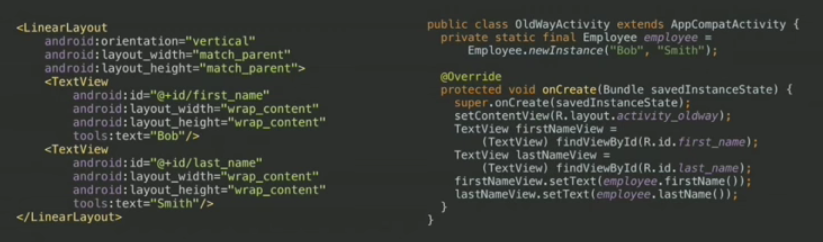
\includegraphics[scale=0.45]{img/DataBinding_vorher}
\caption{Screenshot des Codes wie er ohne Datenanbindung aussieht}
\end{figure}

Ein weitere Umständlichkeit ist es, für jedes Element ein findViewById-casting vornehmen zu müssen, wie wir es im Aktivitätencode vorfinden. Dieses Zugriffsverfahren ist, wie bereits oben erwähnt, unnötig performancelastig und kann vermieden werden.
\subsection{Nacher}

\begin{figure}[h]
\centering
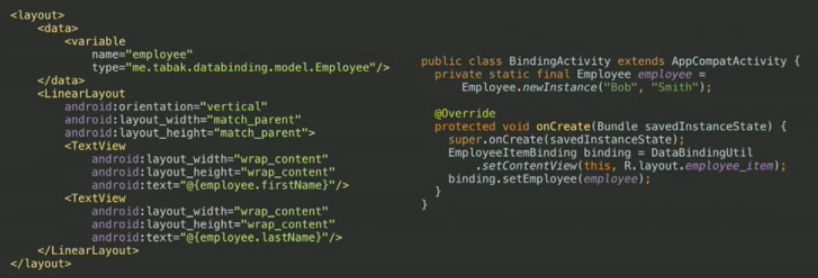
\includegraphics[scale=0.45]{img/DataBinding_nacher}
\caption{Screenshot des Codes wie er mit Datenanbindung aussieht.}
\end{figure}

Auf dieser Grafik sehen wir nun eine Android XML-Layoutdatei mit dem Code in der zugehörigen Aktivität mit der Verwendung von Datenanbindung. Der Unterschied ist, sich keine einzelnen IDs für jedes vorkommende Element mehr ausdenken zu müssen. Ein großer Vorteil ist es, keine findViewById aufrufe mehr machen zu müssen. Man übergibt nur noch das zu bindende Objekt, an dessen Attribute sich die in der Layoutdatei befindenen Elemente orientieren. 
Ein weitere Pluspunkt: Man erkennt sofort für was welches Steuerelement zuständig ist. Ein Programmierer der sich gerade in ein Projekt einarbeitet erkennt sofort, dass bei der ersten TextView der Vorname eines Employeeobjektes angezeigt wird und bei der anderen der Nachname.\footnote{"Droidcon NYC 2015 - Data Binding Techniques" \\ https://www.youtube.com/watch?v=WdUbXWztKNY}

\section{Wie wendet man Datenanbindung an?}
Bei der verwendung von Datenanbindung muss man darauf achten, eine aktuelle Gradle version zu benutzen (min. 1.3). Zusätzlich muss man in der build.gradle (Module App) Datei innerhalb des android\{\}-Bereichs dataBinding auf enabled=true (dataBinding\{enabled=true\}) setzen, um Datenanbindung möglich zu machen.
\subsection{In der .xml Datei}
Gehen wir davon aus, unsere .xml Datei besteht aus einem Linearlayout und zwei TextViews: Remo

\begin{lstlisting}[caption={Layoutcode ohne jedliche Datenanbindung.},label=DescriptiveLabel]
<?xml version="1.0" encoding="utf-8"?>
	<LinearLayout xmlns:android="http://schemas.android.com/apk/res/android"
	android:orientation="vertical"
	android:layout_width="match_parent"
	android:layout_height="match_parent">
		<TextView
			android:id="@+id/vorname"
			android:layout_width="wrap_content"
			android:layout_height="wrap_content"
			android:text="Max" />
		<TextView
			android:id="@+id/nachname"
			android:layout_width="wrap_content"
			android:layout_height="wrap_content"
			android:text="Mustermann" />
</LinearLayout>

\end{lstlisting}

Nun, um Datenanbindung zu ermöglichen, brauchen wir eine Objektklasse auf die wir Referenzieren. In diesem Fall erstellen wir eine Klasse $"$User" mit den String-Attributen firstName und lastName. Die Klasse besteht weiters aus einem Konstruktorfeld mit den Attributen und jeweiliger getter-Felder: 

\begin{lstlisting}[caption={Unsere Objektklasse die bei der Datenanbindung referenziert wird.},label=DescriptiveLabel]
package com.example.daniel.showcasedatabinding;
public class User {
    private final String firstName;
    private final String lastName;

    public User(String firstName, String lastName) {
        this.firstName = firstName;
        this.lastName = lastName;
    }
    public String getFirstName() {
        return this.firstName;
    }
    public String getLastName() {
        return this.lastName;
    }
}
\end{lstlisting}

Haben wir diese erstellt, kann bei der Layoutdatei weitergemacht werden. Wir erstellen nun um unser Layout einen "layout"-Tag. Es folgt ein variable Tag innerhalb eines data Tags. Darin definieren wir eine Variable auf die man innerhalb der Elemente zugreifen kann.

\begin{lstlisting}[caption={Die XML Datei nach der Integration einer Datenanbindung.},label=DescriptiveLabel]
<?xml version="1.0" encoding="utf-8"?>
<layout xmlns:android="http://schemas.android.com/apk/res/android">
    <data>
	    <variable name="user" type="com.example.daniel.showcasedatabinding.User"/>
    </data>
    <LinearLayout
	    android:orientation="vertical"
	    android:layout_width="match_parent"
	    android:layout_height="match_parent">
    
	    <TextView
	        android:layout_width="wrap_content"
	        android:layout_height="wrap_content"
	        android:text="@{user.firstName}" />
		    
	    <TextView
	        android:layout_width="wrap_content"
	        android:layout_height="wrap_content"
	        android:text="@{user.lastName}" />
	    </LinearLayout>
</layout>
\end{lstlisting}


Jetzt können wir unsere ID-Vergabe bei den Elementen löschen und im Text-Tag auf die jeweiligen Attribute des Userobjekts verweisen.

\newpage
\subsection{In der .java Klasse}
Die Datenanbindungstechnologie von Android generiert automatisch spezielle Bindingklasse all jener Layoutdateien die es verwenden. Der Name ergibt sich aus dem Namen der .xml Datei + "binding". Also wenn eine Layoutdatei activity\_main.xml benannt ist, wird daraus die Klasse ActivityMainBinding generiert, die wir nun verwenden können:

\begin{lstlisting}[caption={Die Aktivitätenklasse nach der Integration einer Datenanbindung.},label=DescriptiveLabel]
package com.example.daniel.showcasedatabinding;

import android.databinding.DataBindingUtil;
import android.os.Bundle;
import android.support.v7.app.AppCompatActivity;

import com.example.daniel.showcasedatabinding.databinding.ActivityMainBinding;

public class MainActivity extends AppCompatActivity {

	@Override
	protected void onCreate(Bundle savedInstanceState) {
		super.onCreate(savedInstanceState);

		ActivityMainBinding binding = DataBindingUtil.setContentView(this, R.layout.activity_main);
		User user = new User("Max", "Mustermann");
		binding.setUser(user);
	}
}
\end{lstlisting}

Es wird eine Instanz der generierten Klasse erstellt, welche dann ein Objekt angebunden bekommt, dessen Attribute die Elemente bekommen. Jede Änderung der verwendeten Eigenschaften der erstellten Userinstanz bedeuted auch eine Änderung des Elements, automatisch. \footnote{http://developer.android.com/tools/data-binding/guide.html}

\newpage
\section{Quellen:}
\begin{itemize}
	\item https://www.it-visions.de/
	\item "Droidcon NYC 2015 - Data Binding Techniques" \\ https://www.youtube.com/watch?v=WdUbXWztKNY
	\item http://developer.android.com/tools/data-binding/guide.html
\end{itemize}

\end{document}